\documentclass[fr]{../../../../../../eplexam}

\hypertitle{Automatique linéaire}{6}{INMA}{1510}{2017}{Juin}{Majeure}
{Martin Braquet}
{Denis Dochain}

\section{}
    On a le système suivant :
    \begin{equation*}
        \left \{
        \begin{array}{l @{} l}
            \dot{x} = A x + B u \\
            y = C x \\
        \end{array}
        \right.
        \hspace{0.5cm}
        A = 
        \begin{pmatrix} 
            -1 & 2 & 1 \\
            0 & 1 & -1 \\
            -2 & 4 & 2
        \end{pmatrix}
        \hspace{0.3cm}
        B = 
        \begin{pmatrix} 
            0 \\
            1 \\
            0
        \end{pmatrix}
        \hspace{0.3cm}
        C = 
        \begin{pmatrix} 
            0 & 0 & 1 \\
        \end{pmatrix}
    \end{equation*}
    avec $u(t) = k_1 x_1(t) - k_2 x_2(t) - k_3 x_3(t)$.
    \begin{enumerate}
     \item Comment s'appelle cette structure de commande?
     \item Trouvez les paramètres $k_1$, $k_2$ et $k_3$ pour que la dynamique du système en boucle fermée soit caractérisée par les pôles -1, -4 et -2.
    \end{enumerate}
    Justifiez vos réponses.
    
\begin{solution}
 
\begin{enumerate}
 \item Une commande par retour d'état.
 \item Vérifions tout d'abord si le système est commandable.

Commandabilité ($C_o$): 
$$C_o =  \begin{pmatrix} 
            B & AB & A^2B
        \end{pmatrix} =
         \begin{pmatrix} 
            0 & 2 & 4 \\
            1 & 1 & -3\\
            0 & 4 & 8
        \end{pmatrix}
        $$
    
On remarque que la matrice de commandabilité est de rang 2. En effet la troisième colonne est combili des deux autres ($c_3 = -5c_1+2c_2$). Il y a donc un pôle non commandable, si celui-ci est différent d'un des 3 pôles souhaités, on ne pourra pas assigner la dynamique voulue.

Les valeurs propres de $A$ sont $0$ et $1\pm2i$. Le pôle non commandable est $p=0$ car $$\mathrm{rang}(p\,I-A\quad B)=\mathrm{rang}(-A\quad B)=2<n=3$$
Donc c'est impossible d'assigner des pôles en -1, -2 et -4 puisque le pôle en 0 ne peut pas être déplacé.

\end{enumerate}

\end{solution}

\section{}
    Un patron demande à un des jeunes ingénieurs de régler le régulateur PI d'une de ses installations. Peu expérimenté, ce dernier fouille la littérature et trouve qu'on peut le régler avec la méthode de Cohen-Coon sur bas d'une fonction de transfert simple qui peut être relevée expérimentalement et qui s'écrit comme suit $$G = \frac{K e^{-\theta s}}{\tau s + 1} $$
    Le réglage proposé du régulateur PI est le suivant:
    $$K_p = \dfrac{1}{K} \dfrac{\tau}{\theta}(0.9 + \dfrac{\theta}{12\tau})$$
    $$\tau_i = \dfrac{\theta(30+3\dfrac{\theta}{\tau})}{9+20\dfrac{\theta}{\tau}}$$
    Le jeune ingénieur fait un essai de relevé d'une réponse indicielle sur l'installation. Celle-ci lui permet de déterminer la fonction de transfert, dont les paramètres ont les valeurs suivantes: $K = 0.02$, $\theta = 0.5$, $\tau = 2$.\\
    
    Il applique la méthode de Cohen-Coon, teste les résultats sur son ordinateur et les montre à son patron. Celui-ci n'aparait pas très satisfait. Il lui dit: oiurquoi n'avez-vous pas essayé d'autres méthodes, comme l'ITAE?
    
    Le réglage par la méthode ITAE est le suivant:
    $$K_p = \dfrac{0.586}{K}(\dfrac{\theta}{\tau})^{-0.916}$$
    $$\tau_i = \dfrac{\tau}{1.03 -0.165\dfrac{\theta}{\tau}}$$
    
    Question: analysez le comportement en boucle fermée avec les deux approches et comparez les résultats de votre analyse pour chacune des méthodes. Pouvez-vous expliquer sur cette base le mécontentement du patron? Justifiez votre réponse.\\
    
    Indice: si, dans votre analyse, vous devez approximer un retard, utilisez une forme simple.
    
    \begin{solution}

    Après calcul on à:\\
    $G(s) = \dfrac{0.02}{2s+1}e^{-0.5s}$\\
    $k_{p_{CC}} = 184.167$\\
    $\tau_{i_{CC}} = 1.09821$\\
    $k_{p_{ITAE}} = 104.317$\\
    $\tau_{i_{ITAE}} = 2.0228$\\
    $C_{CC} = \dfrac{184.167(s+0.9106)}{s}$\\
    $C_{ITAE} = \dfrac{104.317(s+0.494375)}{s}$\\
    \\
    L'approximation de Taylor sera utilisé pour cet exercice: $e^{-\theta s} \simeq 1-\theta s$. Trouvons le deux fonction de transfert pour les deux méthodes (on suppose que la rétroaction est unitaire).\\
    \\
    Méthode CC:\\
    \\
    $$Tr(s) = -\dfrac{11.63(s-2)(s+0.91)}{s^2+18.99s+21.18}$$\\
    \\
    Méthode ITAE:\\
    \\
    $$Tr(s) = -\dfrac{1.09(s-2)(s+0.4944)}{s^2+2.69s+1.078}$$\\
    \\
    Les deux fonctions sont stables car $a_1>0$ et $a_2>0$ (condition necessaire et suffisante pour avoir des pôles à partie réelle négative dans une équation d'ordre 2). \\
    Les pôles sont :\\
    \\
    Méthode CC : $p_1 = -17.8$ et $p_2 = -1.19$\\
    \\
    Méthode ITAE : $p_1 = -2.196$ et $p_2 = -0.491$\\
    \\
    Dans un premier temps on peut dire que les pôles de la méthode ITAE sont plus proches de l'axe Imaginaire et donc generent un réponse plus rapide (temps de réponse plus petit)(FAUX). En analysant mieux la méthode ITAE et en faisant une légère approximation on rémarque qu'une annulation pôle-zéro peut être effectuée:\\
    \\
    $0.4944 \simeq 0.491$\\
    $$Tr(s) = \dfrac{1.09(s-2)}{s+2.196}$$\\
    \\
    Cette approximation ne peut pas être faite pour la méthode CC. Ceci veut donc dire que le caractère minimum de phase sera annulé par la méthode ITAE et pas par la méthode CC. En conclusion la réponse de la méthode CC aura un dépassement non négligeable (caractéristique du minimum de phase) et la méthode ITAE sera de premier ordre donc depassement nul.\\
    
    La méthode ITAE est donc meilleure.
    
\end{solution}

\section{}
    Quel contrôleur faut-il employer pour avoir une erreur statique nulle avec une consigne $r(t) = a \sin{\omega t}$? Démontrer.
    
\begin{solution}
 
Imaginons une boucle de rétroaction négative avec un compensateur C(s) sans système G(s) à controller, la consigne est noté r(t) et la sortie y(t). $C_o(s)$ est le numérateur du compensateur. Son degré est toujours inférieur à celui du dénominateur.

Formule générale:
$$ C(s) = \dfrac{1}{s^{q+1}} \prod\limits_{k=1}^p \left(\dfrac{1}{s^2+w_k^2}\right)C_o(s)$$

L'erreur est notée $e(t)$. 
$$y(t)=a\,|Tr(j\omega_0)|\sin\left[\omega_0\,t+\arg(Tr(j\omega_0))\right]$$

$$e_h = 0 \qquad \Longleftrightarrow \qquad Tr(j\omega_0)=1$$

$$\frac{C(j\omega_0)G(j\omega_0)}{1+C(j\omega_0)G(j\omega_0)}=\frac{C_0(j\omega_0)G(j\omega_0)}{(s^2+\omega_0^2)+C_0(j\omega_0)G(j\omega_0)}=1$$
Donc $C(s) = \dfrac{C_o(s)}{(s^2+\omega^2)}$ annule l'erreur statique.

\end{solution}

\section{}
On a la fonction de transfert $G(s) = \dfrac{5 e^{-2 s}}{0.25 s + 1} $.

On souhaite n'avoir qu'un seul pôle en -5.
\begin{enumerate}
    \item Quel contrôleur $C(s)$ faut-il employer? À quoi faut-il faire attention?
    \item En utilisant la même forme de compensateur qu'au point 1, synthétiser un loi de commande qui permette d'éliminer les effets négatifs sur le comportement en boucle fermée. Comment se nomme cette loi de commande? Quelles précautions devez-vous prendre?
    \item Analyser la stabilité en boucle fermée pour les points 1 et 2. Quelles sont vos conclusions?
    \item Pour la deuxième configuration, vous avez fait la synthèse en pensant que le retard était 1 (alors que sa vraie valeur est bien 2). Analysez la stabilité du système en boucle fermée dans ce cas de figure.
\end{enumerate}

Si, à un moment donné de votre démarche, vous devez approximer le retard, utilisez l'approximation de Taylor. 

Justifiez vos réponses.
    
\begin{solution}

\begin{enumerate}
 \item 
    On veut $$Tr(s)=\frac{e^{-2s}}{1+0.2s}$$ 
    Donc $C(s)=\frac{1}{44}\left(1+\frac{4}{s}\right)$.
 
 \item 
    Dans ce paragraphe $G(s)$ est la fonction qui décrit le système sans considèrer le retard $e^{-\theta s}$.
    Une structure de contrôle qui annule les effets du retard n'existe pas. Mais on peut empécher que ce retard sur $G(s)$ ne déstabilise le système grâce à un prédicteur de Smith. Le prédicteur de Smith permet de transférer le retard de $G(s)$ vers la fonction de tranfert $Tr(s)$. Cette structure de contrôle est composée d'un compensateur et un boucle de rétroaction négative non-unitaire de la forme $G(s)(1-e^{-\theta s})$. Le paramètre $\theta$ (le retard) doit être connu à priori sinon le prédicteur de Smith n'est pas optimal. Voici la fonction de transfert d'un prédicteur de Smith:
    $$ C_{Smith}(s) = \dfrac{C(s)}{1+(1-e^{-\theta s})C(s)G(s)}$$
    $$Tr(s) = \dfrac{C_{Smith}(s)G(s)e^{-\theta s}}{1+C_{Smith}(s)G(s)e^{-\theta s}} = \dfrac{C(s)G(s)}{1+C(s)G(s)}e^{-\theta s}$$

    Donc $C(s)=\frac{1}{4}\left(1+\frac{4}{s}\right)$
  
 \item Les 2 systèmes sont stables, tant que l'approximation de Taylor reste valable.
   
 \item C'est pire en sous-évaluant le retard, $Tr(s)$ possède un pôle instable en $p=5/4$ lorsque le retard est sous-évalué à 1.  
\end{enumerate}

\end{solution}

\section{}
On a la fonction de transfert $G = \dfrac{2}{(2 s - 1) ( 5s + 1)} $.

Analyser la stabilité pour ces différents contrôleurs :

\begin{enumerate}
    \item P
    \item PI
    \item PD
    \item PID
\end{enumerate}

\section{}
    On a la structure suivante :
    \begin{center}
        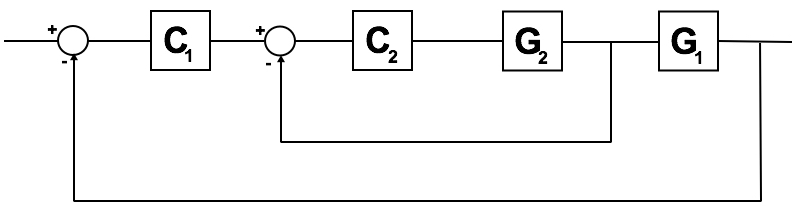
\includegraphics[scale=0.5]{structure.jpg}
    \end{center}
    avec :
    \begin{equation*}
        C_1 = K_{P_1} \dfrac{1 + \tau_i s}{\tau_i s}
        \hspace{0.5cm}
        C_2 = K_{P_2}
        \hspace{0.5cm}
        G_1 = \dfrac{4}{1+4s}
        \hspace{0.5cm}
        G_2 = \dfrac{5}{1+s}
    \end{equation*}
    
    \begin{enumerate}
        \item Quel est le nom de cette structure? Quels sont ses avantages et ses inconvénients?
        \item Trouver les paramètres qui permettent de rendre ce système stable avec uniquement les pôles -4 et -5.
        \item Cette structure permet-elle d'annuler l'erreur statique?
    \end{enumerate}
    Justifiez vos réponses.

\begin{solution}

\begin{enumerate}
    \item 
C'est une structure en cascade. 

Inconvénients : augmente la complexité de la fonction de transfert. 

Avantages : permet de stabiliser d'avantage la fonction de transfert.

    \item 
La démarche pour résoudre cet exercise est la suivante: il faut annuler le(s) pôle(s) avec le(s) zéro(s) (de préférence avec les pôles lents) et ensuite trouver les valeurs qui respectent l'équation de second d'ordre $(s+4)(s+5) = s^2+9s+20$.

La première boucle donne la fonction de transfert suivante :
$$Tr_2(s) = \dfrac{5k_{p_2}}{s+5k_{p_2}+1}$$
On a donc la fonction de transfert suivante :
$$Tr(s) = \dfrac{20 k_{p_1} k_{p_2}(\tau_is+1)}{4\tau_is^3+5(4k_{p_2}+1)\tau_is^2+(20k_{p_1}k_{p_2}+5k_{p_2}+1)\tau_is+20k_{p_1}k_{p_2}}$$
Le dénominateur de cette fonction doit être égal à : $(1 + \tau_i s)(s+4)(s+5) = \tau_is^3+(9\tau_i+1)s^2+(20\tau_i+9)s+20$.
\begin{equation*}
        \left \{
        \begin{array}{l @{} l}
            \dfrac{5}{4}(4k_{p_2}+1) = 9+\dfrac{1}{\tau_i}\\
            -\dfrac{20k_{p_1}k_{p_2}+5k_{p_2}+1}{4}= 20+\dfrac{9}{\tau_i}\\
            -\dfrac{20k_{p_1}k_{p_2}}{4\tau_i}= \dfrac{20}{\tau_i}\\
        \end{array}
        \right.
\end{equation*}

\begin{equation*}
        \left \{
        \begin{array}{l @{} l}
            k_{p_1} = 5/2\\
            k_{p_2} = 8/5\\
            \tau_i= 4\\
        \end{array}
        \right.
\end{equation*}

On aurait pu dès le départ choisir $\tau_1=4$ pour annuler le zéro de $C_1(s)$ avec le pôle de $G_1(s)$.

$$Tr(s) = \dfrac{20}{s^2+9s+20}$$
    
    \item 
L'erreur statique est bien nulle car $Tr(0) = 1$.

\end{enumerate}

\end{solution}

\end{document}
